\documentclass[11pt,a4paper]{article}

\usepackage[T1]{fontenc}
\usepackage[utf8]{inputenc}
\usepackage{newtxtext,newtxmath}
\usepackage{amsmath}
\usepackage[a4paper,margin=25mm,includefoot]{geometry}
\usepackage{microtype}
\usepackage{setspace}
\usepackage{graphicx}
\usepackage{pgfplots}
\usepackage{booktabs}
\usepackage{tabularx}
\usepackage{array}
\usepackage{caption}
\usepackage{enumitem}
\usepackage{float}
\usepackage[section]{placeins}
\usepackage{xcolor}
\usepackage{fancyhdr}
\usepackage{titlesec}
\usepackage{csquotes}
\usepackage[
  backend=biber,
  style=vancouver,
  sorting=none,
  giveninits=true,
  maxbibnames=6,
  minbibnames=3,
  doi=true,
  isbn=false,
  url=false,
  eprint=true
]{biblatex}
\usepackage[hidelinks]{hyperref}
\usepackage[nameinlink,noabbrev]{cleveref}

\addbibresource{references.bib}
\graphicspath{{figures/}}
\pgfplotsset{compat=1.18}

\setstretch{1.08}
\setlength{\parindent}{0pt}
\setlength{\parskip}{0.55em}
\setlength{\emergencystretch}{2em}
\setlength{\headheight}{14pt}
\setcounter{secnumdepth}{2}
\setcounter{tocdepth}{2}

\titleformat{\section}
  {\normalfont\Large\bfseries}{\thesection}{0.65em}{}
\titleformat{\subsection}
  {\normalfont\large\bfseries}{\thesubsection}{0.65em}{}
\titlespacing*{\section}{0pt}{1.2em}{0.45em}
\titlespacing*{\subsection}{0pt}{0.9em}{0.35em}

\captionsetup{
  font=small,
  labelfont=bf,
  justification=centering,
  singlelinecheck=true
}
\renewcommand{\arraystretch}{1.13}

\pagestyle{fancy}
\fancyhf{}
\fancyfoot[C]{\thepage}
\renewcommand{\headrulewidth}{0pt}

\hypersetup{
  pdftitle={Development and Evaluation of an Evidence-Grounded Multimodal RAG System for Scientific Literature},
  pdfauthor={Kang Wu},
  pdfsubject={MSc Advanced Mechanical Engineering Final Report},
  pdfkeywords={retrieval-augmented generation, multimodal learning, scientific literature, information retrieval, evidence grounding}
}

\DeclareFieldFormat{doi}{%
  doi\addcolon\space
  \href{https://doi.org/#1}{\nolinkurl{#1}}%
}

\newcolumntype{Y}{>{\raggedright\arraybackslash}X}
\newcommand{\code}[1]{\texttt{\detokenize{#1}}}

\begin{document}

\begin{titlepage}
\thispagestyle{empty}
\centering
\setlength{\fboxsep}{12pt}
\fbox{%
\begin{minipage}[t][0.82\textheight][t]{0.88\textwidth}
\centering
\vspace{0.6cm}
{\Large\bfseries University of Birmingham\par}
{\Large College of Engineering and Physical Sciences\par}
\vspace{0.8cm}
{\Large\bfseries Department of Mechanical Engineering\par}
{\Large School of Engineering\par}
\vspace{0.9cm}
{\Large MSc Advanced Mechanical Engineering\par}
\vspace{0.8cm}
{\LARGE\bfseries Advanced Project\par}
\vspace{0.45cm}
{\Large\bfseries 2025--26 Session\par}
\vspace{0.75cm}
{\LARGE\bfseries FINAL REPORT\par}
\vspace{0.75cm}

\renewcommand{\arraystretch}{1.55}
\begin{tabularx}{0.96\linewidth}{|>{\raggedright\arraybackslash}p{0.27\linewidth}|Y|}
\hline
Surname & \textbf{Wu} \\ \hline
First Name & \textbf{Kang} \\ \hline
ID number & \textbf{3035412} \\ \hline
Supervisor's Name & \textbf{Jiaqi Ye} \\ \hline
Project Title & \textbf{Development and Evaluation of an Evidence-Grounded Multimodal RAG System for Scientific Literature} \\ \hline
\end{tabularx}
\end{minipage}}
\end{titlepage}

\setcounter{page}{2}

\begin{center}
{\LARGE\bfseries Development and Evaluation of an Evidence-Grounded Multimodal RAG System for Scientific Literature\par}
\vspace{0.35em}
\rule{\linewidth}{0.5pt}
\end{center}

\section*{Abstract}

Scientific answers need traceable evidence, especially when relevant full texts require institutional access. This project evaluated a multimodal retrieval-augmented generation (RAG) system over a locally managed corpus covering ultrasound, thermal ablation, thermometry and thermal imaging. It combined provenance-preserving PDF ingestion, lexical and dense retrieval, rank fusion, CrossEncoder reranking, Gemini generation and image summaries. The corpus contained 272 papers, 3,904 page records and 4,243 chunks; DOI metadata was present for 82.94\% of chunks and 5.28\% had an unknown section. A fixed 50-question development/evaluation set assigned one source chunk to each question. The author checked every label against its source and online record before a Codex consistency check; 32 were approved and 18 corrected. Because the set informed configuration comparison and lacked medical-specialist review, it remains non-expert silver data rather than an independent test benchmark. Hybrid source-paper Recall@5 was 0.62, compared with 0.56 for lexical and 0.52 for dense retrieval; lexical-pool reranking produced the highest mean reciprocal rank (MRR), 0.605. A 350-word/50-overlap ablation achieved source-paper Recall@5 of 0.74 but created 64.9\% more chunks than production 650/90. Across 30 answerable and ten evidence-insufficient questions, a fixed Gemini judge scored grounded hybrid RAG at 1.867/2 for correctness and faithfulness, with 97.6\% citation precision, complete abstention and a 2.0\% unsupported-claim rate, down from 26.9\% without evidence. These are LLM-judged estimates, not expert clinical scores. The multimodal extension converted images into Gemini Vision observations and retrieval terms before the existing text retriever; it did not use a joint image--text index. On 12 figures, vision summaries did not improve source Recall@5 beyond 0.917 or produce a detectable quality difference. The multimodal findings remain exploratory and do not constitute clinical validation.

\noindent\textbf{Keywords:} retrieval-augmented generation; multimodal learning; scientific literature; information retrieval; evidence grounding

\FloatBarrier
\section{Introduction}
\label{sec:introduction}

Large language models (LLMs) can explain scientific topics fluently without providing reliable evidence. They may rely on training data, combine incompatible experiments or produce a plausible statement that cannot be traced to a publication. This is a practical problem in ultrasound thermometry, thermal ablation and thermal imaging, where methods differ in maturity, range and setting. A research answer must therefore link back to its paper, page and passage.

Access creates a second problem. University subscriptions provide full texts that public tools may not index, so a general chatbot can miss papers available to a Birmingham researcher. Uploading subscription papers to an external service can also raise copyright and governance concerns. A controlled local corpus limits bulk document transfer and preserves provenance, although selected excerpts still leave the device when an external generator is used.

Retrieval-augmented generation (RAG) separates knowledge storage from generation by supplying retrieved passages as context. Lewis et al. improved several knowledge-intensive tasks with a retrievable Wikipedia index \cite{lewis2020rag}. RAG still permits parsing, retrieval and generation failures, so evaluation must examine each stage rather than one opaque answer score.

This project aims to develop and evaluate a multimodal RAG system over a locally managed private corpus for evidence-grounded question answering on institution-accessible scientific literature concerning ultrasound, thermal ablation, thermometry, high-intensity focused ultrasound (HIFU) and thermal imaging. The work has six technical objectives:

\begin{enumerate}[leftmargin=*,itemsep=0.2em]
\item construct a traceable research corpus with document identifiers and bibliographic metadata;
\item extract text from scientific PDFs while preserving page and section context;
\item create retrieval-ready chunks with controlled size and overlap;
\item compare lexical, dense and hybrid retrieval, followed by CrossEncoder reranking;
\item generate English answers constrained by retrieved evidence, with numbered citations and explicit uncertainty; and
\item extend and evaluate the system for exploratory image-grounded questions without claiming clinical interpretation.
\end{enumerate}

These objectives lead to four research questions (RQs). RQ1 asks how lexical, dense, hybrid and reranked retrieval trade off evidence recall, ranking quality and latency on the project corpus. RQ2 examines how chunk size and overlap affect early evidence retrieval. RQ3 asks how retrieved evidence and reranking affect answer correctness, faithfulness, completeness, citation support and abstention when compared with generation without retrieval. RQ4 tests whether a question-aware visual summary improves source retrieval and grounded answering when compared with a text-only question or basic image metadata.

The resulting artefact is a FastAPI application with a Vite and React interface, SQLite storage, SentenceTransformers embeddings, hybrid retrieval, CrossEncoder reranking, Gemini generation and a question-aware image analysis path. The contribution is an auditable implementation and component-level evaluation on a specialised corpus, not a new foundation model. Generator fine-tuning would not fix failures in corpus quality, retrieval or prompting.

\FloatBarrier
\section{Literature Review and State of the Art}
\label{sec:literature-review-and-state-of-the-art}

\subsection{Retrieval-augmented generation and evidence grounding}
\label{sec:retrieval-augmented-generation-and-evidence-grounding}

Lewis et al. reported more specific and factual output than a parametric-only baseline \cite{lewis2020rag}. Their Wikipedia experiments do not directly solve scientific-document QA, where papers are long, heterogeneous and conditional. This work therefore exposes intermediate evidence rather than treating RAG as a guarantee against hallucination.

Hallucination is treated as content that conflicts with, or is unsupported by, supplied evidence. LLMs can produce and fail to recognise it \cite{li2023halueval}, because unconstrained generation does not establish evidential truth \cite{bouyamourn2023hallucinate}. Retrieval reduces this risk only when context is relevant and used faithfully \cite{es2024ragas}. The prompt therefore requires numbered citations, clearly separated visual observations and abstention; code rejects citation indices outside the supplied sources.

\subsection{Sparse, dense and hybrid retrieval}
\label{sec:sparse-dense-and-hybrid-retrieval}

BM25 provides a term-weighted lexical signal \cite{robertson2009bm25}. Dense Passage Retrieval outperformed BM25 on several open-domain QA datasets \cite{karpukhin2020dpr}, while Sentence-BERT made independently encoded text practical for similarity search \cite{reimers2019sbert}. Their relative value in this specialist corpus is tested rather than assumed.

Hybrid retrieval combines these signals. RRF operates on rank positions rather than raw scores \cite{cormack2009rrf}. This project compares it with weighted fusion because its FTS and dense scores are not naturally calibrated.

A dual encoder permits precomputed corpus vectors but scores query and passage independently. A CrossEncoder models their interaction more closely and is therefore used to rerank only a limited candidate pool. Lexical, dense and hybrid pools are tested separately because reranking cannot recover evidence omitted by the first stage.

\subsection{Scientific PDF parsing, chunking and metadata}
\label{sec:scientific-pdf-parsing-chunking-and-metadata}

Scientific PDF extraction depends on visual layout. VILA improves structured extraction with line or block groups \cite{shen2022vila}, while cross-layout tests show degradation under publisher and layout-distribution shifts \cite{chen2023layout}. Nougat instead uses visual OCR to reconstruct scientific markup \cite{blecher2023nougat}. This prototype uses deterministic PyMuPDF extraction and preserves title, DOI, year, page, section and chunk ID for audit.

Short passages can lose document-level context and depend strongly on split choice \cite{liu2021dense}; simply retaining more text is not sufficient because models can miss evidence in the middle of long contexts \cite{liu2024lost}. Four sizes and overlaps are therefore evaluated rather than assuming a universal default.

This system indexes titles and sections as retrieval fields, while DOI, page and chunk identifiers form its audit trail. SciRepEval shows that scientific representations can struggle to generalise across classification, regression, ranking and search formats \cite{singh2023scirepeval}; performance on this corpus is therefore measured directly.

\subsection{RAG evaluation}
\label{sec:rag-evaluation}

End-to-end correctness cannot locate a failure. RAGAS separates context, faithfulness and answer quality \cite{es2024ragas}; ARES combines synthetic judge training with a small human-labelled set \cite{saadfalcon2024ares}. A healthcare review found no standardised RAG evaluation framework \cite{amugongo2025healthcare}. This study therefore separates retrieval, citation and repeated LLM judging over non-expert silver labels.

Recall@k records whether labelled evidence appears in the first k results; MRR emphasises its first rank, and nDCG rewards relevant sources near the top. Generation is assessed for correctness, faithfulness, completeness, abstention, unsupported claims and citation support.

\subsection{Multimodal scientific retrieval}
\label{sec:multimodal-scientific-retrieval}

CLIP established transferable image--text alignment, and BLIP improved visual understanding and caption generation \cite{radford2021clip,li2022blip}. SciMMIR nevertheless reports a scientific-domain gap because figure captions commonly express results or principles rather than generic scenes \cite{wu2024scimmir}. The implementation therefore uses Gemini Vision to produce question-aware observations and retrieval terms for the audited text retriever; it does not build a separate visual index.

The extension distinguishes visual observations from literature evidence and does not infer calibrated temperature from pixels without radiometric metadata. Questions use captions and context rather than diagnosis; source images are not redistributed, and figure credits are checked separately. MR, ultrasound and infrared thermometry also remain acquisition-, tissue- or protocol-dependent \cite{mattay2024mr,lena2021interleaved,rohfritsch2024ultrasound,ring2012infrared,lahiri2012medical,stanley2024acute}. The evaluation is therefore exploratory literature retrieval, not clinical validation.

\FloatBarrier
\section{Methodology and System Design}
\label{sec:methodology-and-system-design}

\subsection{Research design and frozen system}
\label{sec:research-design-and-frozen-system}

Figure~\ref{fig:architecture} summarises the frozen architecture evaluated in this study.

\begin{figure}[tbp]
  \centering
  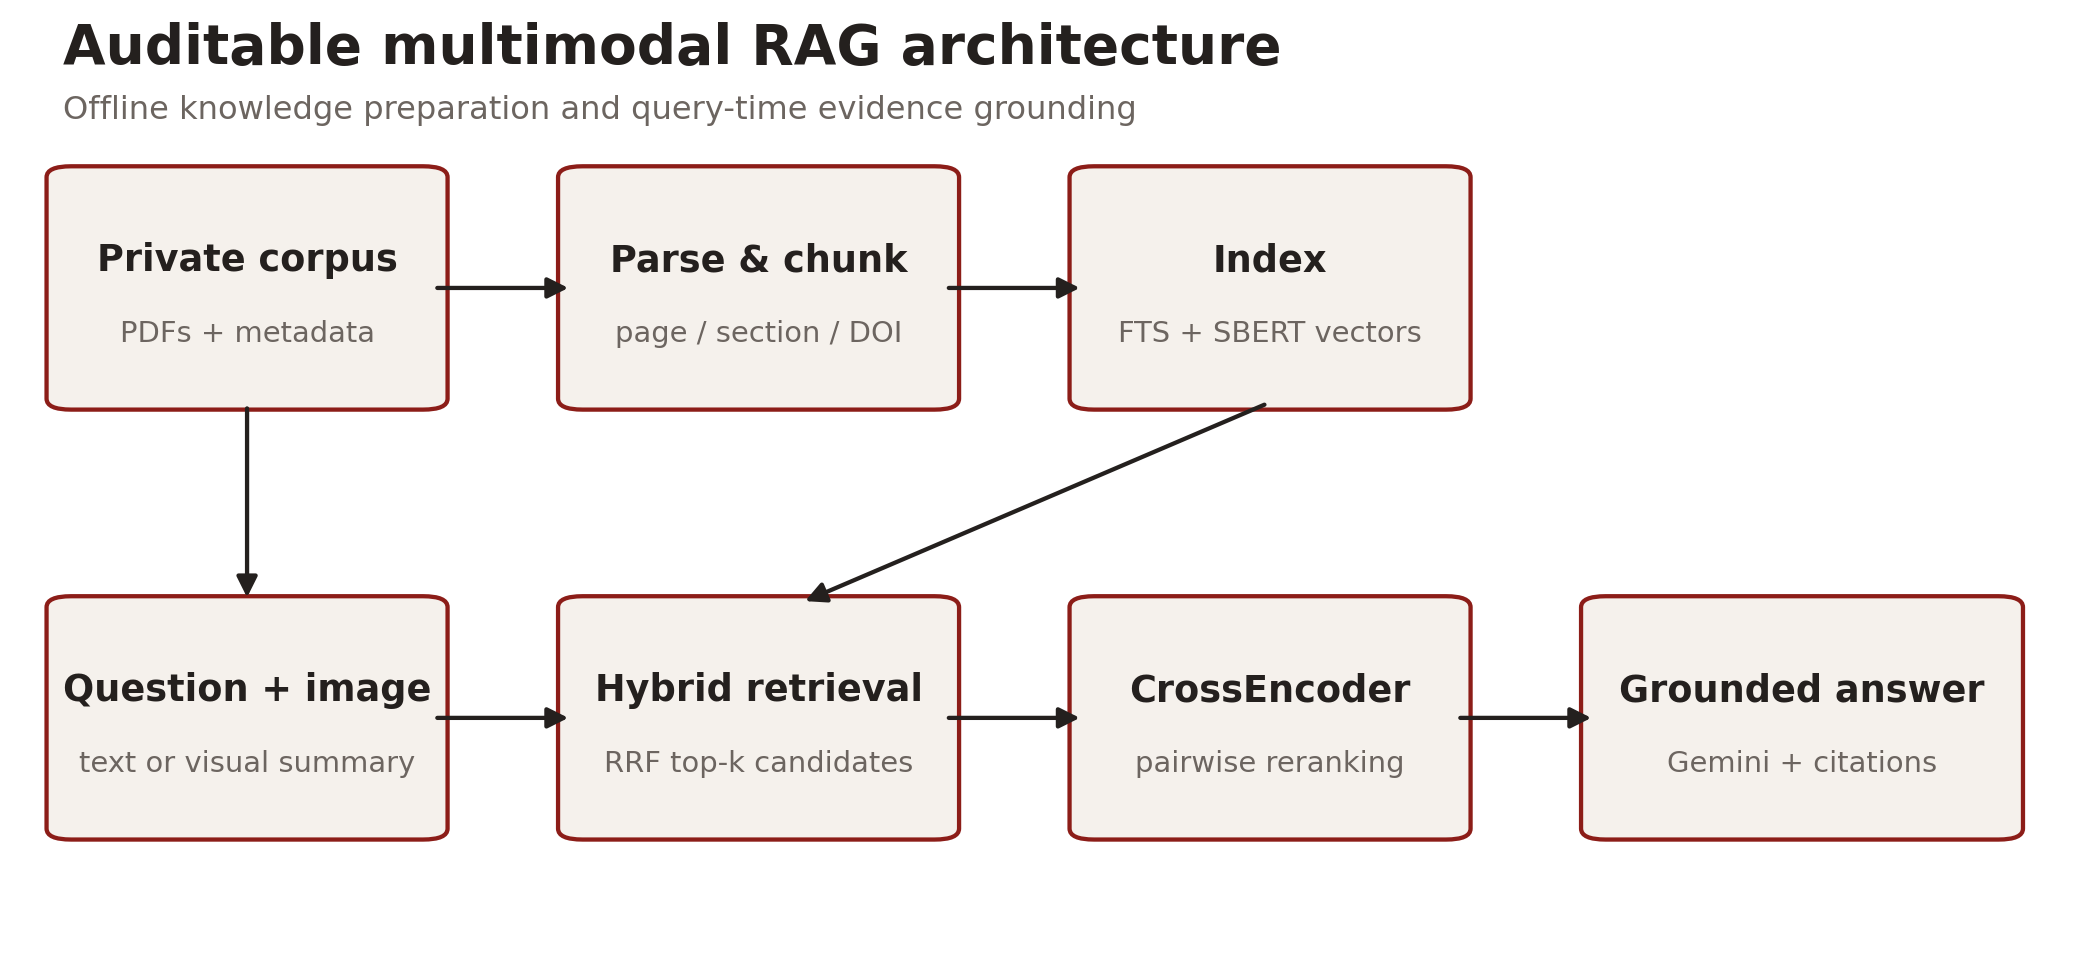
\includegraphics[width=0.96\linewidth]{figure-1-architecture.png}
  \caption{Auditable multimodal RAG architecture evaluated in this study.}
  \label{fig:architecture}
\end{figure}

Artefact development was followed by controlled comparative evaluation. The application was frozen at commit \code{e416772}, tag \code{image-qa-v1-2026-06-23}; interfaces and tested parameters were not changed in response to results. Each run recorded the commit, seed, models, parameters, per-case output, summary and latency in an immutable directory.

The system comprises FastAPI, Vite/React, SQLite and modular ingestion, retrieval, generation and image services. Evaluation concerns the evidence pipeline rather than UI appearance. Corpus files and embeddings remain local; query-time Gemini calls transmit selected evidence excerpts or the requested image, so the prototype is locally managed but not fully on-premises.

Figure~\ref{fig:demo-interface} shows the final demonstration interface and its evidence cards.

\begin{figure}[tbp]
  \centering
  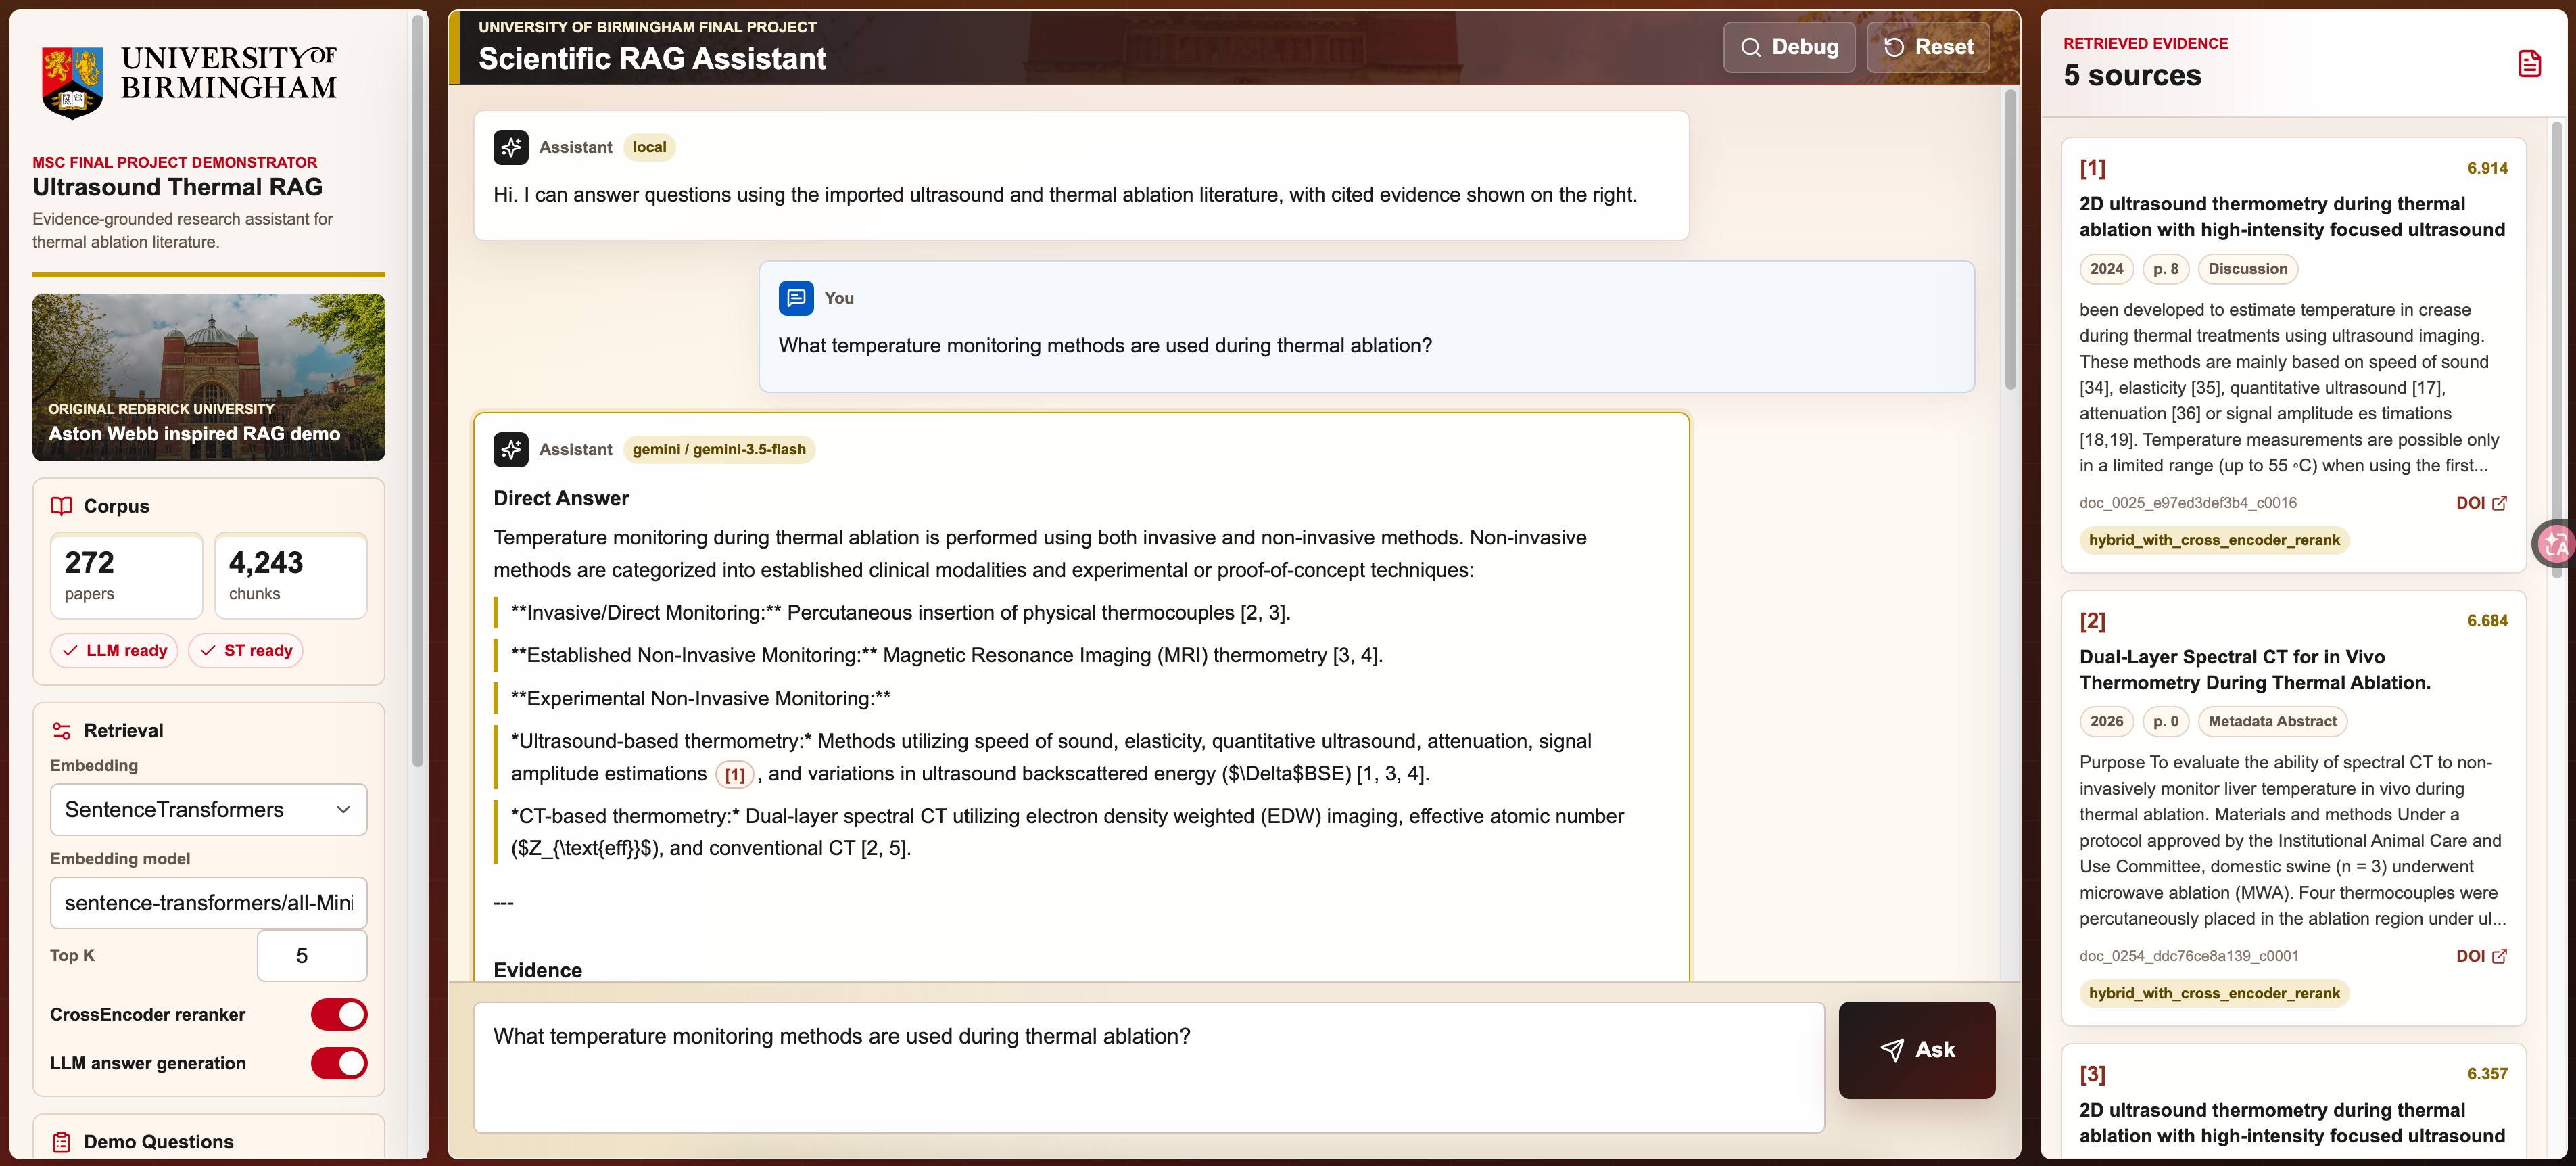
\includegraphics[width=\linewidth]{figure-6-demo.png}
  \caption{Demonstration interface with grounded answer and retrieved evidence cards.}
  \label{fig:demo-interface}
\end{figure}

\subsection{Corpus construction and technical audit}
\label{sec:corpus-construction-and-technical-audit}

Table~\ref{tab:corpus-audit} summarises the corpus construction and parsing audit.

\begin{table}[tbp]
  \centering
  \caption{Corpus construction and parsing audit.}
  \label{tab:corpus-audit}
  \small
  \begin{tabularx}{\linewidth}{@{}l l Y@{}}
    \toprule
    \textbf{Component} & \textbf{Count / coverage} & \textbf{Audit note} \\
    \midrule
    Documents & 272 & All PDFs present \\
    Page records & 3,904 & Page-level provenance \\
    Chunks & 4,243 & Production 650/90 configuration \\
    DOI metadata & 82.94\% & Not all sources assign a DOI \\
    Unknown section & 5.28\% & Parser limitation \\
    Visual sample & 30 documents / 524 pages & 5 approved; 21 minor; 4 rebuild \\
    \bottomrule
  \end{tabularx}
\end{table}

The source snapshot was collected on 28 May 2026 through OpenAlex, Europe PMC, arXiv and lawful publisher/repository links. Candidates required a readable, relevant PDF; duplicate DOI, inherited-key and PDF-hash records were consolidated. The build contained 272 papers from 2004--2026, including 13 obtained through authorised institutional access and kept local.

Records retained source, access and extraction metadata. PyMuPDF extracted text, coordinates and images; chunks preserved page, section and stable IDs. Corpus chunks used 650-word maximum, 120-word minimum and 90-word overlap. The separate 900/150-character upload splitter was not evaluated.

The audit checked extraction, metadata, empty text, replacement characters, short chunks and \code{Unknown} sections; repeated boundary lines were flagged as possible headers or footers. In a deterministic sample stratified by age and length, all 524 physical pages from 30 PDFs were rendered and inspected for page coverage, reading order, section metadata, table/equation linearisation and false reference boundaries. This author-led technical audit used automated flags and Codex anomaly cross-checks; it was neither clinical nor independent expert review.

\subsection{Retrieval configurations}
\label{sec:retrieval-configurations}

The 50-question set was constructed after corpus indexing from a fixed, Codex-assisted list of topic specifications covering applications, methods, mechanisms, risks, parameters, comparisons and facts. Each specification defined required or optional terms and preferred sections. A deterministic script scored the 4,243 chunks, discouraged repeated use of one document, selected the highest-scoring unused chunk and extracted up to two supporting sentences. All questions were answerable; each had exactly one nominated chunk and source paper, and together they covered 40 documents. Alternative valid passages or papers were not exhaustively labelled.

The author checked every question, answer and passage against local primary-source text and an online publication record before a Codex consistency check. Thirty-two labels were approved and 18 corrected by narrowing scope, completing an answer or replacing weak evidence; none was deleted. The same fixed set was then used to compare retrieval, reranking, metadata and chunk configurations and to inspect errors. It is therefore a development/evaluation set, not an untouched hold-out. It did not train or fine-tune SentenceTransformers, the CrossEncoder or Gemini. All comparisons retained the same order and seed 3035412. Without medical-specialist review, the process improves traceability but not expert validity.

Full-text search in SQLite FTS supplied the lexical/BM25-style baseline. Dense retrieval used \path{sentence-transformers/all-MiniLM-L6-v2}; 384-dimensional corpus embeddings were precomputed and cosine similarity was evaluated locally. The model is compact enough for a laptop and requires no inference API key.

Two fusion methods were compared. RRF combined lexical and dense ranks using Equation~\eqref{eq:rrf}:
\begin{equation}
\label{eq:rrf}
\operatorname{RRF}(d)=\sum_{r\in\{\mathrm{lex},\mathrm{dense}\}}
\frac{1}{60+\operatorname{rank}_{r}(d)} .
\end{equation}
Weighted fusion was tested at lexical weights 0.50 and 0.75. Candidate pools contained up to 80 passages. CrossEncoder experiments used \path{cross-encoder/ms-marco-MiniLM-L-6-v2}, sequence length 384, batches of 16 and the first 900 characters per candidate. Lexical, dense and RRF pools were reranked separately; sensitivity tests varied reranker-pool size and indexed metadata.

Metrics were Recall@5, @10 and @20, mean reciprocal rank (MRR), normalised discounted cumulative gain (nDCG) at 5 and 10, and end-to-end query latency. Every label supplied one chunk ID, document ID and DOI where available. Matching used an OR rule: an exact chunk match or any returned chunk with the same document ID or normalised DOI counted as a hit. The reported Recall, MRR and nDCG are therefore source-paper metrics, not strict supporting-passage metrics. A correct paper can still expose the wrong passage to the generator, while other valid passages or papers may be unlabelled. MRR used \(1/r_i\) for the first source-paper hit, with zero for a miss; nDCG discounted that hit by rank. Per-question ranks were retained for paired error analysis.

\subsection{Chunk ablation}
\label{sec:chunk-ablation}

Four word-based chunk configurations were reconstructed from the same page records: 350 words with 50-word overlap, the production 650/90 configuration, 650/0 and 900/150. Section and page boundaries were retained where possible. For comparability, every condition used the same questions, SentenceTransformer model, lexical index construction, RRF algorithm, candidate pool and evaluation metrics. The number and mean length of generated chunks were reported because apparent retrieval improvements can require a much larger index.

\subsection{Generation and citation evaluation}
\label{sec:generation-and-citation-evaluation}

Thirty answerable reviewed-silver questions were selected proportionally by type with a fixed seed; ten designed evidence-insufficient questions tested abstention. Three conditions were compared.

\textbf{Condition A (no retrieval):} Gemini without retrieved evidence.

\textbf{Condition B (dense RAG):} dense-vector retrieval with the top five passages.

\textbf{Condition C (hybrid grounded RAG):} RRF hybrid retrieval, CrossEncoder reranking and a grounded prompt with the top five passages.

Condition C represented the intended production architecture. It was retained because RRF combined lexical and semantic signals and had broader first-stage source-paper Recall@5 than lexical retrieval (0.62 versus 0.56). Lexical-pool reranking achieved the highest MRR, so hybrid plus reranking is not claimed to be the empirically optimal ranker. The choice reflects an engineering trade-off informed by the same development/evaluation set, not independent held-out validation.

The grounded prompt required direct answer, evidence, limitations, \code{Sources used}, a \code{[n]} marker for literature claims and abstention when evidence was insufficient. Because no sources were supplied to the no-retrieval baseline, citation precision was not applicable to that condition.

Programmatic checks validated only citation syntax and index range. A fixed-schema Gemini judge scored answerable-case correctness, faithfulness and completeness (0--2), and assessed claims, semantic citation support, unsupported claims and abstention. Two temperature-zero judgements were retained for each answer. Unsupported-claim rate used all cases; citation precision used answerable grounded cases; abstention accuracy used only evidence-insufficient cases. These semantic metrics are LLM-judged estimates, not independent expert truth.

\subsection{Exploratory image question answering}
\label{sec:exploratory-image-question-answering}

From seven CC BY 4.0 corpus papers, a technical screen selected 12 complete-caption figures: four ultrasound/thermometry, four thermal-distribution and four schematic/quantitative plots. The manifest recorded source, page, figure, caption and expected document. The author checked source pages, captions, credit lines and licences online before using Codex to cross-check the records. Ten figures had no special credit; one PLOS composite used prior-study photographs, and one BioRender schematic required separate confirmation. All 12 figures were restricted to internal evaluation and excluded from the report and public package; the two flagged figures were additionally marked unsuitable for public reproduction without figure-specific confirmation. No identifying or diagnostic task was included.

Three conditions used the same question for each image.

\textbf{Condition A (text only):} the text question without image-derived input.

\textbf{Condition B (basic metadata):} the question plus locally computed dimensions, format and uncalibrated pixel statistics.

\textbf{Condition C (vision summary):} the question plus a Gemini Vision summary constrained to observable features, uncertainty and retrieval terms.

Gemini Vision first converted each image into textual observations and retrieval terms; those terms extended the question sent to the same text-based hybrid/CrossEncoder pipeline. No joint image--text embedding or direct image-index retrieval was used. Source Recall@5 tested paper retrieval; caption coverage, citation quality, structure, unsupported visual inference and contradiction assessed answers. Captions can omit visible details and are not independent clinical labels.

\subsection{Software verification and analysis}
\label{sec:software-verification-and-analysis}

Evaluation used an Apple M1 MacBook Air (8 GB), macOS 15.2 and Python 3.10.6; the final verification suite passed all 27 tests. Selection used seed 3035412 and resampling seed 20260723. Ninety-five per cent bootstrap intervals used 10,000 resamples; paired two-sided randomisation tests used 50,000 sign swaps at \(\alpha=0.05\). The \(p\)-values were unadjusted across multiple exploratory comparisons: \emph{nominally detectable} means unadjusted \(p<0.05\). Interpretation therefore prioritises effect sizes and confidence intervals. These tests quantify case-sampling uncertainty, not label error or external generalisation.

\FloatBarrier
\section{Results}
\label{sec:results}

\subsection{Corpus and parsing quality}
\label{sec:corpus-and-parsing-quality}

The automated audit found 272 PDFs, 3,904 page records and 4,243 chunks. DOI coverage was 82.94\%; provenance fields were complete. It found 224 \code{Unknown}-section chunks (5.28\%), 16 short chunks, no replacement characters and 339 possible repeated boundary lines.

The screen found 5 approved, 21 minor, and 4 rebuild cases. False reference boundaries omitted body text in two papers, while two had unreliable formula/table extraction. The sample identifies failure types, not a corpus-wide error rate.

\subsection{Retrieval and reranking}
\label{sec:retrieval-and-reranking}

Figure~\ref{fig:retrieval-results} compares retrieval and reranking performance.

\begin{figure}[tbp]
  \centering
  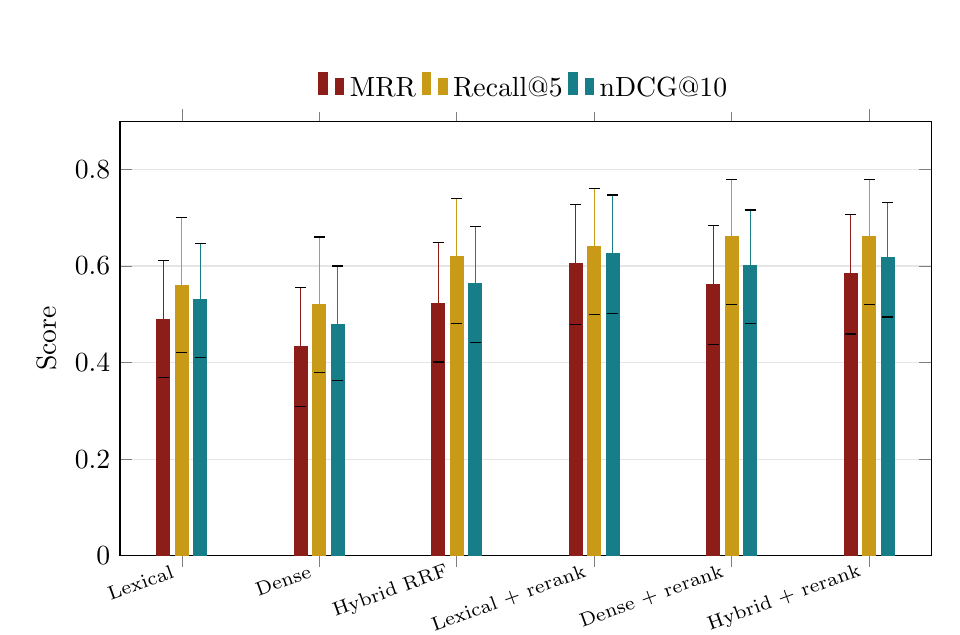
\begin{tikzpicture}
    \begin{axis}[
      ybar,
      width=0.98\linewidth,
      height=7.1cm,
      ymin=0,
      ymax=0.90,
      ylabel={Score},
      xtick={0,1,2,3,4,5},
      xticklabels={Lexical,Dense,Hybrid RRF,Lexical + rerank,Dense + rerank,Hybrid + rerank},
      x tick label style={font=\scriptsize,rotate=20,anchor=east},
      ymajorgrids=true,
      grid style={gray!20},
      bar width=4.7pt,
      enlarge x limits=0.09,
      legend style={at={(0.5,1.02)},anchor=south,legend columns=-1,draw=none},
      legend cell align=left
    ]
      \addplot[draw={rgb,255:red,140;green,29;blue,24},fill={rgb,255:red,140;green,29;blue,24},error bars/.cd,y dir=both,y explicit]
      table[x=x,y=y,y error plus=upper,y error minus=lower] {
        x y upper lower
        0 0.4886 0.1223 0.1192
        1 0.4326 0.1229 0.1234
        2 0.5230 0.1257 0.1218
        3 0.6052 0.1230 0.1263
        4 0.5622 0.1213 0.1256
        5 0.5842 0.1222 0.1250
      };
      \addplot[draw={rgb,255:red,201;green,154;blue,24},fill={rgb,255:red,201;green,154;blue,24},error bars/.cd,y dir=both,y explicit]
      table[x=x,y=y,y error plus=upper,y error minus=lower] {
        x y upper lower
        0 0.56 0.14 0.14
        1 0.52 0.14 0.14
        2 0.62 0.1205 0.14
        3 0.64 0.12 0.14
        4 0.66 0.12 0.14
        5 0.66 0.12 0.14
      };
      \addplot[draw={rgb,255:red,23;green,126;blue,137},fill={rgb,255:red,23;green,126;blue,137},error bars/.cd,y dir=both,y explicit]
      table[x=x,y=y,y error plus=upper,y error minus=lower] {
        x y upper lower
        0 0.5296 0.1175 0.1199
        1 0.4791 0.1210 0.1155
        2 0.5632 0.1185 0.1224
        3 0.6257 0.1213 0.1239
        4 0.6002 0.1159 0.1197
        5 0.6165 0.1149 0.1221
      };
      \legend{MRR,Recall@5,nDCG@10}
    \end{axis}
  \end{tikzpicture}
  \caption{Source-paper retrieval and reranking performance; error bars show 95\% bootstrap confidence intervals.}
  \label{fig:retrieval-results}
\end{figure}

Lexical MRR and Recall@5 were 0.489 and 0.56; dense retrieval reached 0.433 and 0.52. RRF was the strongest mode before reranking: MRR 0.523 (95\% CI 0.401--0.649), Recall@5 0.62 (0.480--0.741) and Recall@20 0.74. Relative to dense retrieval, RRF had nominally higher MRR by 0.090 (unadjusted \(p=0.000060\)) and nDCG@10 by 0.084 (unadjusted \(p=0.000140\)); its Recall@5 difference was not nominally detectable. No RRF--lexical difference was nominally detectable, so the result does not establish universal hybrid superiority.

Lexical reranking raised MRR to 0.605 (unadjusted \(p=0.031959\)) and nDCG@10 to 0.626 (unadjusted \(p=0.034299\)); both changes were nominally detectable. RRF reranking gave MRR 0.584 and nDCG@10 0.617, but neither change was nominally detectable. Reranking therefore reordered supplied candidates but could not recover first-stage omissions.

Mean latency was 25.3 ms for lexical, 36.4 ms for dense, 62.0 ms for RRF and 321--341 ms with CrossEncoder. Pool-size and indexed-metadata sensitivity tests produced no nominally detectable difference.

Table~\ref{tab:retrieval-errors} converts per-question ranks into an automated screening taxonomy. It identifies where to inspect, rather than proving a root cause.

\begin{table}[tbp]
  \centering
  \caption{Automated retrieval screening over 50 reviewed-silver questions.}
  \label{tab:retrieval-errors}
  \small
  \begin{tabularx}{\linewidth}{@{}l r Y Y@{}}
    \toprule
    \textbf{Pattern} & \textbf{n} & \textbf{Observation} & \textbf{Next action} \\
    \midrule
    Candidate omission & 13 & Outside top 30 & Rewrite query \\
    Reranker demotion & 2 & Top-five hit moved down & Train reranker \\
    Context cutoff & 2 & Ranked 6--30 & Expand context \\
    Later promotion & 6 & Fusion/reranker rescue & Retain stages \\
    Single-stage hit & 7 & Lexical or dense only & Retain hybrid \\
    Shared success & 20 & All core stages hit & None \\
    \bottomrule
  \end{tabularx}
\end{table}

\subsection{Chunk ablation}
\label{sec:chunk-ablation-2}

Figure~\ref{fig:chunk-ablation} shows the early-recall and index-size trade-off.

\begin{figure}[tbp]
  \centering
  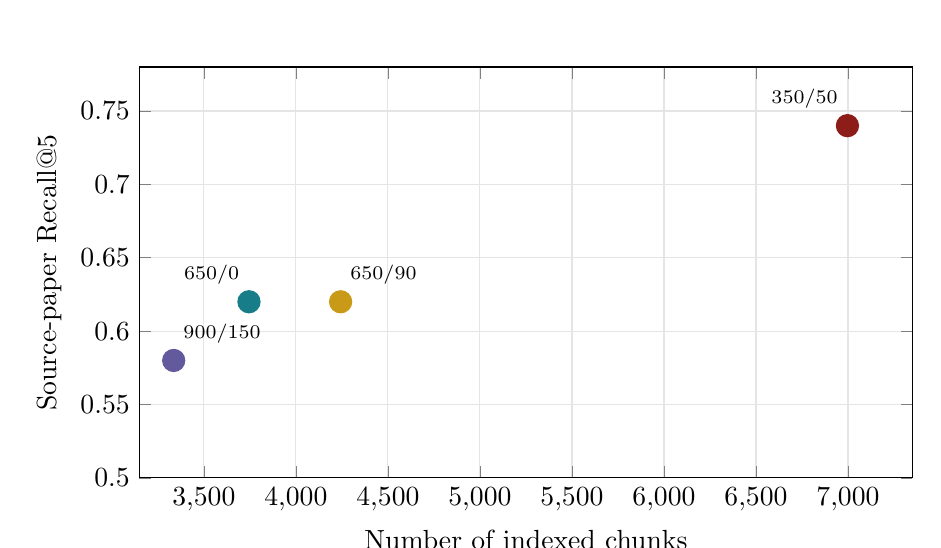
\begin{tikzpicture}
    \begin{axis}[
      width=0.94\linewidth,
      height=6.8cm,
      xmin=3150,
      xmax=7350,
      ymin=0.50,
      ymax=0.78,
      xlabel={Number of indexed chunks},
      ylabel={Source-paper Recall@5},
      grid=major,
      grid style={gray!20}
    ]
      \addplot[only marks,mark=*,mark size=4pt,color={rgb,255:red,140;green,29;blue,24}] coordinates {(6997,0.74)};
      \addplot[only marks,mark=*,mark size=4pt,color={rgb,255:red,201;green,154;blue,24}] coordinates {(4243,0.62)};
      \addplot[only marks,mark=*,mark size=4pt,color={rgb,255:red,23;green,126;blue,137}] coordinates {(3745,0.62)};
      \addplot[only marks,mark=*,mark size=4pt,color={rgb,255:red,98;green,90;blue,156}] coordinates {(3336,0.58)};
      \node[anchor=south east,font=\scriptsize] at (axis cs:6997,0.745) {350/50};
      \node[anchor=south west,font=\scriptsize] at (axis cs:4243,0.625) {650/90};
      \node[anchor=south east,font=\scriptsize] at (axis cs:3745,0.625) {650/0};
      \node[anchor=south west,font=\scriptsize] at (axis cs:3336,0.585) {900/150};
    \end{axis}
  \end{tikzpicture}
  \caption{Source-paper Recall@5 and index-size trade-off across chunk configurations.}
  \label{fig:chunk-ablation}
\end{figure}

The 350/50 condition created 6,997 chunks and achieved the best MRR (0.574), Recall@5 (0.74) and nDCG@10 (0.618). Production 650/90 created 4,243 chunks and reached 0.523, 0.62 and 0.563. Its differences from 350/50 were nominally detectable for all three metrics (unadjusted \(p=0.043599\), 0.031219 and 0.019900). The smaller chunks improved early recall by 12 points but enlarged the index by 64.9\%; production is a resource compromise, not the observed retrieval optimum.

\subsection{Generation and citation}
\label{sec:generation-and-citation}

Gemini-judged generation, faithfulness and abstention results are summarised in Table~\ref{tab:generation-results} and Figure~\ref{fig:generation-results}.

\begin{table}[tbp]
  \centering
  \caption{Gemini-judged generation quality on 30 answerable cases, unsupported-claim rate on all 40 cases, and abstention on ten evidence-insufficient cases.}
  \label{tab:generation-results}
  \small
  \begin{tabular}{@{}lccccc@{}}
    \toprule
    \textbf{Mode} & \textbf{Correct.} & \textbf{Faithful.} & \textbf{Complete.} & \textbf{Unsupported} & \textbf{Abstention} \\
    \midrule
    LLM only & 1.467 & 1.633 & 1.400 & 0.269 & 0.700 \\
    Dense RAG & 1.767 & 1.867 & 1.833 & 0.020 & 1.000 \\
    Hybrid reranked RAG & 1.867 & 1.867 & 1.933 & 0.020 & 1.000 \\
    \bottomrule
  \end{tabular}
\end{table}

\begin{figure}[tbp]
  \centering
  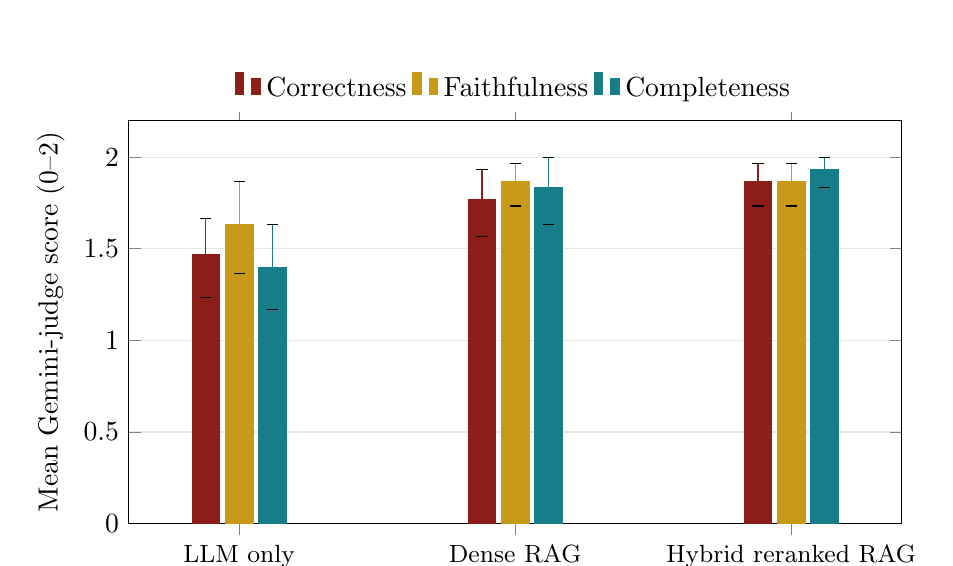
\begin{tikzpicture}
    \begin{axis}[
      ybar,
      width=0.94\linewidth,
      height=6.7cm,
      ymin=0,
      ymax=2.2,
      ylabel={Mean Gemini-judge score (0--2)},
      xtick={0,1,2},
      xticklabels={LLM only,Dense RAG,Hybrid reranked RAG},
      x tick label style={font=\small,align=center},
      ymajorgrids=true,
      grid style={gray!20},
      bar width=10pt,
      enlarge x limits=0.2,
      legend style={at={(0.5,1.02)},anchor=south,legend columns=-1,draw=none},
      legend cell align=left
    ]
      \addplot[draw={rgb,255:red,140;green,29;blue,24},fill={rgb,255:red,140;green,29;blue,24},error bars/.cd,y dir=both,y explicit]
      table[x=x,y=y,y error plus=upper,y error minus=lower] {
        x y upper lower
        0 1.4667 0.2000 0.2334
        1 1.7667 0.1666 0.2000
        2 1.8667 0.1000 0.1334
      };
      \addplot[draw={rgb,255:red,201;green,154;blue,24},fill={rgb,255:red,201;green,154;blue,24},error bars/.cd,y dir=both,y explicit]
      table[x=x,y=y,y error plus=upper,y error minus=lower] {
        x y upper lower
        0 1.6333 0.2334 0.2666
        1 1.8667 0.1000 0.1334
        2 1.8667 0.1000 0.1334
      };
      \addplot[draw={rgb,255:red,23;green,126;blue,137},fill={rgb,255:red,23;green,126;blue,137},error bars/.cd,y dir=both,y explicit]
      table[x=x,y=y,y error plus=upper,y error minus=lower] {
        x y upper lower
        0 1.4000 0.2333 0.2333
        1 1.8333 0.1667 0.2000
        2 1.9333 0.0667 0.1000
      };
      \legend{Correctness,Faithfulness,Completeness}
    \end{axis}
  \end{tikzpicture}
  \caption{Mean Gemini-judged generation scores under the three evidence conditions; error bars show 95\% bootstrap confidence intervals.}
  \label{fig:generation-results}
\end{figure}

The Gemini judge scored the no-retrieval baseline at mean correctness 1.467/2, faithfulness 1.633 and completeness 1.400 on answerable questions. Its judged unsupported-claim rate was 26.9\% across all cases (95\% CI 10.9--43.8\%), and judged abstention was correct on 70\% of ten evidence-insufficient questions. No out-of-range citation marker was detected.

The judge scored dense RAG at 1.767 for correctness, 1.867 for faithfulness and 1.833 for completeness; judged unsupported claims fell to 2.0\% (0.5--4.0\%), semantic citation precision was 98.2\% (96.0--100\%) and abstention accuracy was 100\%. Hybrid reranked RAG scored 1.867, 1.867 and 1.933; the corresponding values were 2.0\% (0.5--4.1\%), 97.6\% (95.2--99.4\%) and 100\%. Relative to no retrieval, dense RAG had nominally higher judged completeness (unadjusted \(p=0.021560\)); hybrid RAG had nominally higher judged correctness (unadjusted \(p=0.010020\)) and completeness (unadjusted \(p=0.000120\)). Faithfulness differences and all hybrid--dense differences were not nominally detectable.

The answer model was \code{gemini-3.5-flash-lite}. All 120 answers received two temperature-zero structured judgements from the fixed \code{gemini-3.6-flash} judge, producing 240 judgements. Exact repeat agreement and quadratic weighted kappa were 1.0 for every mode and metric, demonstrating deterministic reproducibility rather than independent validity. Amortised batched generation latency was approximately 0.95--1.00 s per answer and is not equivalent to single-user UI latency.

\subsection{Exploratory image QA}
\label{sec:exploratory-image-qa}

Table~\ref{tab:image-qa-results} and Figure~\ref{fig:image-qa-results} report the exploratory image-QA comparison.

\begin{table}[tbp]
  \centering
  \caption{Gemini-judged exploratory image-QA results on 12 figures from seven CC BY 4.0 articles.}
  \label{tab:image-qa-results}
  \small
  \begin{tabular}{@{}lccccc@{}}
    \toprule
    \textbf{Mode} & \textbf{Source R@5} & \textbf{Caption} & \textbf{Citation} & \textbf{Structure} & \textbf{Contradictions} \\
    \midrule
    Text only & 0.917 & 1.583 & 1.833 & 1.917 & 0 \\
    Basic metadata & 0.917 & 1.750 & 1.833 & 2.000 & 0 \\
    Vision summary & 0.917 & 1.750 & 1.917 & 2.000 & 0 \\
    \bottomrule
  \end{tabular}
\end{table}

\begin{figure}[tbp]
  \centering
  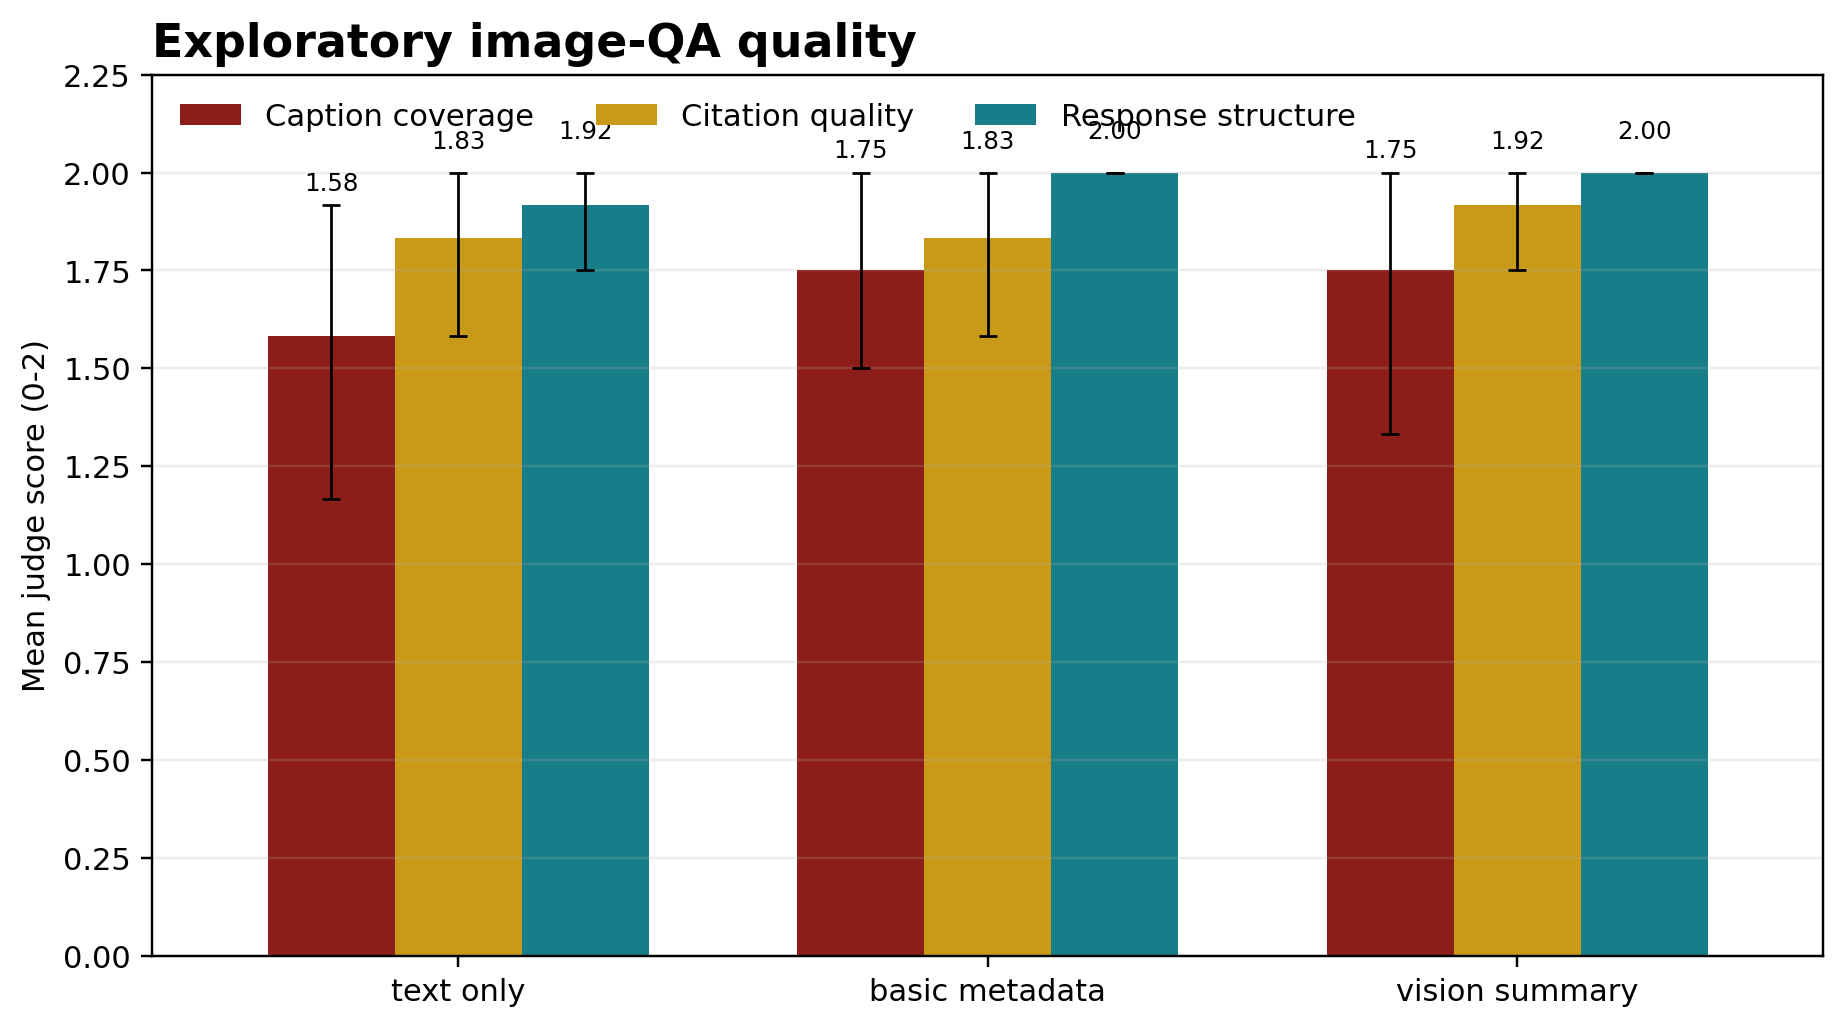
\includegraphics[width=0.94\linewidth]{figure-5-image-qa.png}
  \caption{Gemini-judged image-QA quality; error bars show 95\% bootstrap confidence intervals.}
  \label{fig:image-qa-results}
\end{figure}

Source Recall@5 was 0.917 (95\% CI 0.75--1.00) in all conditions. The Gemini judge scored text-only caption coverage at 1.583/2 and vision summary at 1.750, with vision citation quality 1.917. No vision comparison was nominally detectable.

The judge counted three unsupported visual inferences for text-only answers, one with basic metadata and none with the vision summary; no contradiction or invalid citation index occurred. These are sample findings, not proof of zero risk. Vision summarisation added 5.41 s per image.

\FloatBarrier
\section{Discussion}
\label{sec:discussion}

\subsection{Interpretation of retrieval results}
\label{sec:interpretation-of-retrieval-results}

RRF increased Recall@5 by 0.06 over lexical and 0.10 over dense search, supporting the literature distinction between exact term matching and semantic representation \cite{robertson2009bm25,karpukhin2020dpr,reimers2019sbert}. Its MRR and nDCG@10 gains over dense retrieval were nominally detectable with very small unadjusted \(p\)-values, whereas no RRF--lexical difference was detected. The result supports rank fusion for this corpus \cite{cormack2009rrf}, not a universal claim that hybrid retrieval is superior.

CrossEncoder reranking produced nominal lexical-pool gains in MRR and nDCG@10 while Recall@20 changed little, consistent with reordering within a fixed candidate pool. Candidate omission remained the largest failure category. The final hybrid/CrossEncoder path retained wider first-stage source-paper coverage and both retrieval signals, whereas lexical-pool reranking maximised MRR. This is an engineering trade-off, not evidence that the final path was optimal.

The 350/50 index produced nominal gains in MRR, Recall@5 and nDCG@10 but expanded storage by 65\%. The literature identifies two related risks: splitting can remove document context, while longer input does not guarantee evidence use \cite{liu2021dense,liu2024lost}. Metadata did not uniformly improve dense retrieval, so future work should test section weighting and neighbouring-chunk expansion rather than assume prefixes are beneficial.

\subsection{Generation, citation and hallucination}
\label{sec:generation-citation-and-hallucination}

Grounding reduced unsupported claims and improved abstention. Its nominal gains concerned correctness or completeness, not faithfulness, and hybrid reranking did not outperform dense RAG. This supports component-level evaluation advocated by RAGAS and ARES \cite{es2024ragas,saadfalcon2024ares}. Reviewed-silver labels and a Gemini-family judge still prevent claims of scientific correctness.

External evidence does not eliminate hallucination \cite{li2023halueval,bouyamourn2023hallucinate,amugongo2025healthcare}. A generator can attach a valid index to the wrong claim or overgeneralise an experiment. Code verifies citation syntax and range, not semantic entailment; independent sentence-level review remains necessary.

\subsection{Multimodal interpretation}
\label{sec:multimodal-interpretation}

The image experiment did not support the hypothesis that a visual summary would increase source Recall@5. Caption-derived questions created a ceiling effect, consistent with the gap between generic image--language tasks \cite{radford2021clip,li2022blip} and scientific-figure retrieval \cite{wu2024scimmir}. No quality difference was nominally detectable; the feature's present value is explicit observation and uncertainty, not higher retrieval accuracy, at 5.4 s additional latency.

Separating observations from literature claims is useful, but summary errors can influence retrieval and generation. Captions are not independent labels because they guided the questions. Future work should add independent questions, panel crops, axis/legend OCR and scientific image-text embeddings.

\subsection{Threats to validity}
\label{sec:threats-to-validity}

The 50 questions were constructed from the indexed corpus and reused for configuration comparison and error analysis, so the reported performance is not an independent held-out estimate. Each question has one nominated chunk rather than exhaustive relevance judgements; a valid unlisted paper may be counted wrong, while source-paper matching can reward a returned chunk that lacks the required sentence. Author review and Codex cross-checking do not make these expert gold labels or establish clinical validity.

Thirty answerable cases and 12 images support comparison, not biomedical generalisation. Designed unanswerable questions may make abstention easier. Gemini-family judging introduces rubric and family bias; repeated temperature-zero outputs measure reproducibility, not human agreement. Multiple unadjusted exploratory tests increase false-positive risk, so effect sizes and confidence intervals take priority.

Audit metrics are proxies: complete fields need not be correct. The author-led 524-page screen, with automated flags and Codex cross-checking, exposed false reference stops, coarse sections and damaged table/equation structure, but 30 documents cannot establish a corpus-wide error rate. Scientific PDFs remain vulnerable to layout errors \cite{shen2022vila,chen2023layout}; rights and institutional-access conditions also require continuing review.

Latency was measured on one Apple computer after loading, not under multi-user load. API latency and quotas remain provider- and network-dependent.

\subsection{Objective traceability}
\label{sec:objective-traceability}

Table~\ref{tab:objective-traceability} shows how each objective is evidenced rather than inferred from the interface.

\begin{table}[H]
  \centering
  \caption{Objective traceability.}
  \label{tab:objective-traceability}
  \small
  \begin{tabularx}{\linewidth}{@{}l Y Y@{}}
    \toprule
    \textbf{Objective} & \textbf{Method / result evidence} & \textbf{Conclusion} \\
    \midrule
    O1 corpus & ID/metadata audit & 272-paper traceable corpus \\
    O2 parsing & 30 PDFs / 524-page screen & 26 usable; 4 require rebuild \\
    O3 chunking & Four-condition ablation & 650/90 trades size for recall \\
    O4 retrieval & Retrieval/reranking tests & Fusion broadens; reranking reorders \\
    O5 grounding & 40-question test & Unsupported claims reduced \\
    O6 multimodal & 12-figure comparison & Exploratory, not validated \\
    \bottomrule
  \end{tabularx}
\end{table}

\FloatBarrier
\section{Impact Statement}
\label{sec:impact-statement}

The project offers students and researchers an auditable way to explore specialised literature. Users can inspect each passage, title, DOI, page and chunk identifier rather than accept an uncited answer. This may reduce initial evidence-finding time and include authorised institution-accessible papers without incorporating them into model parameters.

Stakeholders include postgraduate researchers, supervisors, research groups, librarians, IT teams, authors and publishers; patients could be harmed by unvalidated clinical use.

Deployment should remain research-oriented and require authentication, encrypted storage, document-level licence rules, audit logs, deletion procedures and corpus review. Benefits should be measured through evidence-finding time, retrieval coverage and citation support, not clinical outcomes. Although embeddings are local, selected excerpts and images reach Gemini; prompts should therefore contain only necessary evidence.

Potential economic value lies in research time saved, while deployment adds storage, API, maintenance and rights-management costs. Environmental effects were not measured; local inference reduces some transfer, but model computation and storage still consume energy.

Risks include copyright misuse, confidential data, automation bias, incomplete literature, false citations and visual over-interpretation. Controls include authorised acquisition, open-licence evaluation images, no patient identifiers, explicit uncertainty, evidence cards, citation checks and no diagnosis or treatment recommendations. Scientific accountability remains with the researcher.

\FloatBarrier
\section{Conclusions}
\label{sec:conclusions}

This project produced an auditable multimodal RAG demonstrator over 272 papers and 4,243 provenance-preserving chunks. For RQ1, no configuration dominated every criterion. RRF offered the strongest pre-reranking source-paper trade-off at 62 ms (Recall@5 0.62), while lexical-pool CrossEncoder reranking achieved the highest MRR, 0.605, at 341 ms. The final hybrid/CrossEncoder path retained broader first-stage source coverage and both retrieval signals; it is not claimed as the MRR optimum.

For RQ2, 350/50 produced the highest Recall@5, 0.74, but 65\% more chunks than production; its MRR, Recall@5 and nDCG@10 gains were nominally detectable. The selected 650/90 configuration is therefore a resource compromise rather than an optimum.

For RQ3, the Gemini judge estimated that grounding reduced unsupported claims from 26.9\% to approximately 2.0\%, abstained correctly on all ten evidence-insufficient cases and achieved 97.6--98.2\% citation precision. It found nominal correctness and completeness gains, but no faithfulness or hybrid--dense difference; these are not expert clinical scores. For RQ4, the vision-to-text extension did not improve source Recall@5 beyond 0.917 or produce a detectable quality difference. It remains an exploratory query-expansion method, not a direct joint image--text retriever. Future work should prioritise corpus, passage-level retrieval and expert evaluation.

\FloatBarrier
\section*{Acknowledgements}

The author thanks Dr Jiaqi Ye for project supervision and feedback. Codex supported implementation, evaluation scripts, metadata and literature checks, figure and LaTeX preparation, and language revision. Google Gemini provided answer generation, vision summaries and structured judging. Their outputs were checked against source code, saved experiments and cited primary publications; responsibility for the submitted work remains with the author.

\FloatBarrier
\printbibliography[title={References}]

\clearpage
\appendix
\section{Abbreviations and Symbols}
\label{sec:abbreviations}

\small
\renewcommand{\arraystretch}{1.06}
\begin{tabularx}{\linewidth}{@{}>{\bfseries}p{0.16\linewidth}Y@{}}
API & application programming interface. \\
BM25 & Best Matching 25 probabilistic lexical ranking function. \\
BLIP & Bootstrapping Language--Image Pre-training. \\
CC BY & Creative Commons Attribution licence. \\
CI & confidence interval. \\
CLIP & Contrastive Language--Image Pre-training. \\
DOI & digital object identifier. \\
FTS & full-text search. \\
HIFU & high-intensity focused ultrasound. \\
IRT & infrared thermography. \\
LLM & large language model. \\
MR/MRI & magnetic resonance/magnetic resonance imaging. \\
MRR & mean reciprocal rank. \\
nDCG & normalised discounted cumulative gain. \\
PDF & Portable Document Format. \\
PRFS & proton resonance frequency shift. \\
QA & question answering. \\
RAG & retrieval-augmented generation. \\
RQ & research question. \\
RRF & reciprocal rank fusion. \\
SBERT & Sentence-BERT. \\
SciMMIR & Scientific Multi-Modal Information Retrieval. \\
TA & thermoacoustic. \\
UST & ultrasound tomography. \\
Recall@k & proportion of questions with labelled evidence in the first \emph{k} results. \\
top-k & the first \emph{k} ranked retrieval results. \\
\end{tabularx}
\normalsize

\section{Reproducibility and Review Boundary}
\label{sec:reproducibility-review}

The evaluated software state is Git commit \code{e416772}, tag \code{image-qa-v1-2026-06-23}. Runs record models, parameters, seeds, input hashes, per-case output, summaries and latency. Privacy-safe source code and reproducibility materials are available at \url{https://github.com/ChrisWu11/multimodal-rag}; private PDFs, evidence text, source figures, embeddings, the database, local paths and API credentials are excluded.

Completed checks include the corpus audit, confidence intervals, paired tests, citation-index validation, verification of all 25 references, article-level licence checks and source-page rights checks for 12 figures. Bibliographic identity does not prove claim support, and an article licence does not prove that every panel is original.

The 50-label review recorded 32 approvals and 18 corrections; expert sign-off remains separate. The PDF audit found 5 approved, 21 minor, and 4 rebuild cases. All source figures were excluded from public release. The module permits the declared use of Codex and Gemini, but wording remains the author's responsibility. No patient-identifying data are processed, and the system is not a clinical decision tool.

\end{document}
